\documentclass[10pt, tikz, border=12pt]{standalone}
\usepackage{helvet}
\renewcommand{\familydefault}{\sfdefault}
\usepackage{amsmath,amssymb}
\usepackage{tikz}
\usetikzlibrary{positioning, fit, calc, arrows.meta, shapes.geometric, decorations.pathreplacing, backgrounds}

\definecolor{emeraldpine}{HTML}{1A4D3E}
\definecolor{harvardcrimson}{HTML}{A51C30}
\definecolor{ethdarkblue}{HTML}{1F407A}
\definecolor{ethpetrol}{HTML}{007A87}
\definecolor{ethbronze}{HTML}{B87333}
\definecolor{ethpurple}{HTML}{5B4B8A}
\definecolor{ink}{HTML}{1A202C}
\definecolor{softink}{HTML}{4A5568}
\definecolor{paleink}{HTML}{A0AEC0}
\definecolor{cardbg}{HTML}{F8FAFC}
\definecolor{shadecolor}{HTML}{F4F6F9}

\begin{document}
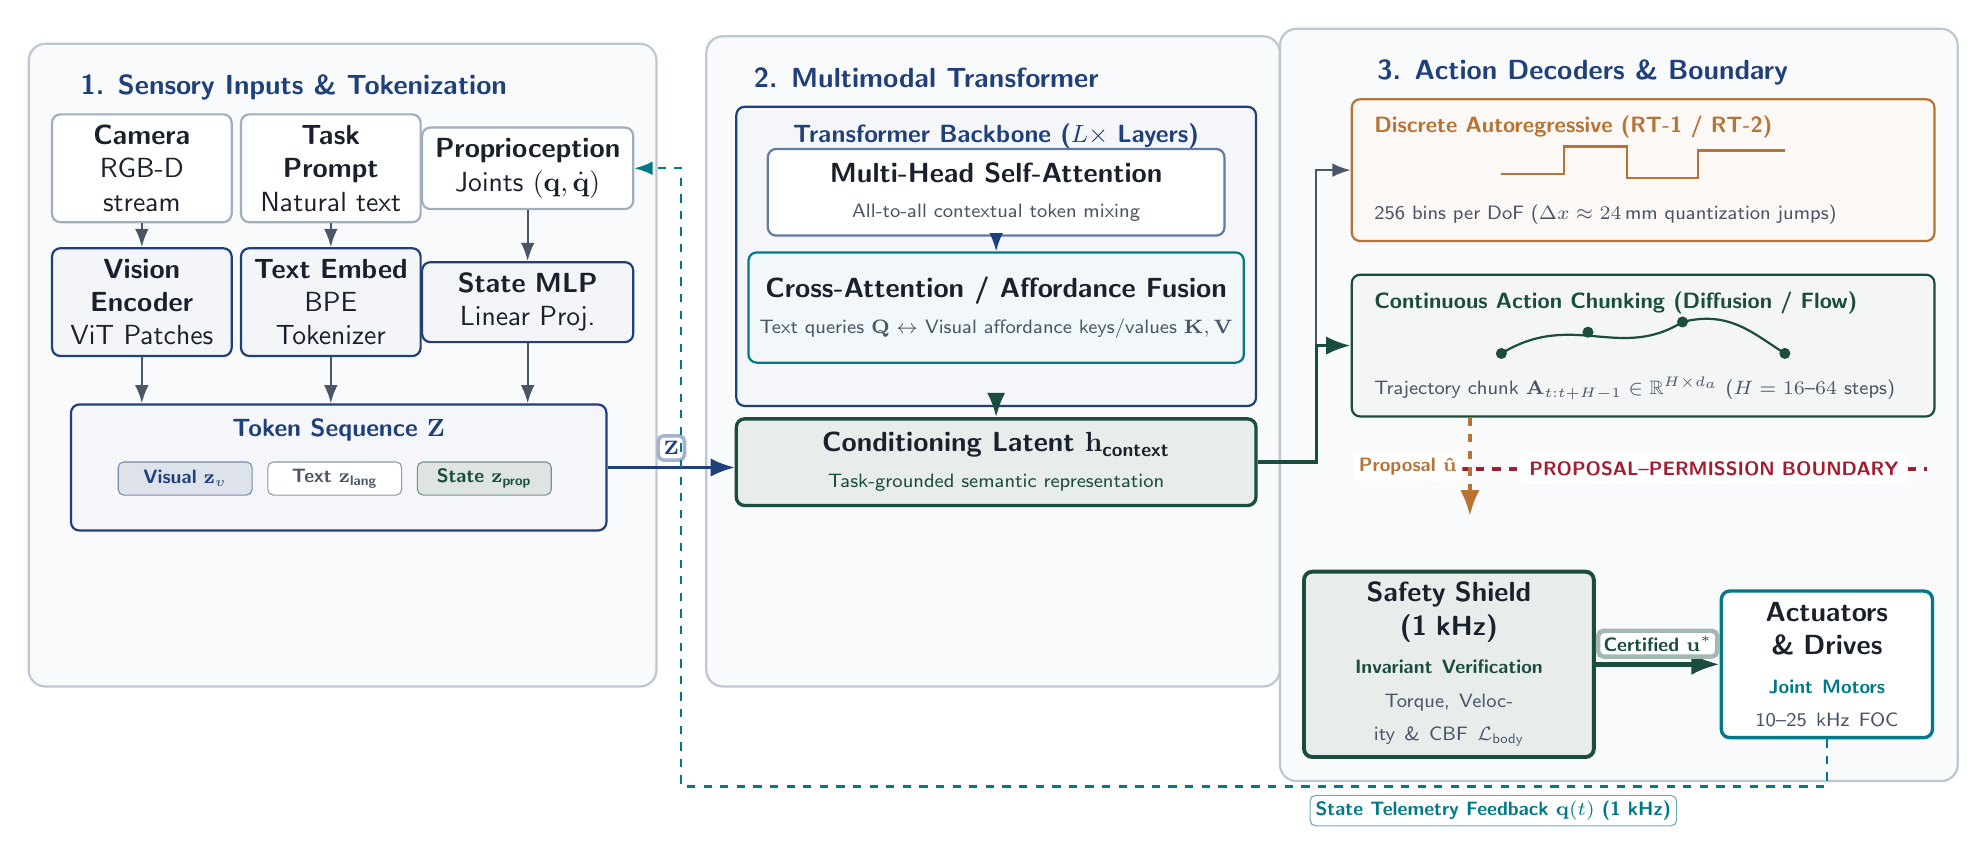
\begin{tikzpicture}[
    >=Latex,
    font=\sffamily,
    box/.style={draw=paleink, fill=white, rounded corners=3pt, inner sep=4pt, align=center, text=ink, thick},
    colheader/.style={font=\sffamily\bfseries\color{ethdarkblue}, anchor=north west},
    colbg/.style={draw=paleink!70, fill=cardbg, rounded corners=6pt, thick},
    arrow/.style={->, thick, draw=ethdarkblue},
    arr_slate/.style={->, thick, draw=softink},
    arr_prop/.style={->, thick, draw=ethbronze},
    signal/.style={font=\sffamily\scriptsize, fill=white, inner sep=2pt, rounded corners=2pt}
]

% ================= COLUMN 1: SENSORY INPUTS & TOKENIZATION =================
\coordinate (col1_nw) at (0, 0.8);
\node[colheader] (col1_title) at (0.2, 0.6) {1. Sensory Inputs \& Tokenization};

% 1A: Raw Inputs
\node[box, text width=2.0cm] (cam_in) at (1.1, -0.7) {\textbf{Camera}\\RGB-D stream};
\node[box, text width=2.0cm] (lang_in) at (3.5, -0.7) {\textbf{Task Prompt}\\Natural text};
\node[box, text width=2.4cm] (prop_in) at (6.0, -0.7) {\textbf{Proprioception}\\Joints $(\mathbf{q}, \dot{\mathbf{q}})$};

% 1B: Token Embedding Blocks
\node[box, draw=ethdarkblue, fill=ethdarkblue!5, text width=2.0cm] (cam_emb) at (1.1, -2.4) {\textbf{Vision Encoder}\\ViT Patches};
\node[box, draw=ethdarkblue, fill=ethdarkblue!5, text width=2.0cm] (lang_emb) at (3.5, -2.4) {\textbf{Text Embed}\\BPE Tokenizer};
\node[box, draw=ethdarkblue, fill=ethdarkblue!5, text width=2.4cm] (prop_emb) at (6.0, -2.4) {\textbf{State MLP}\\Linear Proj.};

\draw[arr_slate] (cam_in) -- (cam_emb);
\draw[arr_slate] (lang_in) -- (lang_emb);
\draw[arr_slate] (prop_in) -- (prop_emb);

% 1C: Unified Token Sequence Z
\node[box, draw=ethdarkblue, fill=shadecolor, minimum width=6.8cm, minimum height=1.6cm] (tokens) at (3.6, -4.5) {};
\node[anchor=north, font=\sffamily\small\bfseries\color{ethdarkblue}, yshift=-2pt] at (tokens.north) {Token Sequence $\mathbf{Z}$};

% Token chips inside Sequence Z
\begin{scope}[shift={($(tokens.center) + (-2.8, -0.35)$)}]
    \draw[fill=ethdarkblue!15, draw=ethdarkblue!60, rounded corners=2pt] (0,0) rectangle (1.7, 0.42);
    \node[font=\scriptsize\bfseries\color{ethdarkblue}] at (0.85, 0.21) {Visual $\mathbf{z}_v$};
    
    \draw[fill=white, draw=softink!60, rounded corners=2pt] (1.9,0) rectangle (3.6, 0.42);
    \node[font=\scriptsize\bfseries\color{softink}] at (2.75, 0.21) {Text $\mathbf{z}_{\text{lang}}$};
    
    \draw[fill=emeraldpine!15, draw=emeraldpine!60, rounded corners=2pt] (3.8,0) rectangle (5.5, 0.42);
    \node[font=\scriptsize\bfseries\color{emeraldpine}] at (4.65, 0.21) {State $\mathbf{z}_{\text{prop}}$};
\end{scope}

\draw[arr_slate] (cam_emb) -- (cam_emb |- tokens.north);
\draw[arr_slate] (lang_emb) -- (lang_emb |- tokens.north);
\draw[arr_slate] (prop_emb) -- (prop_emb |- tokens.north);

\coordinate (col1_bot) at (3.6, -7.0);

% Background bounding box for column 1
\begin{scope}[on background layer]
    \node[colbg, fit=(col1_title) (cam_in) (prop_in) (tokens) (col1_bot), inner sep=8pt] (col1_bg) {};
\end{scope}

% ================= COLUMN 2: MULTIMODAL TRANSFORMER BACKBONE =================
\coordinate (col2_nw) at ($(col1_bg.north east) + (0.9cm, 0)$);
\node[colheader] (col2_title) at ($(col2_nw) + (0.2, -0.2)$) {2. Multimodal Transformer};

% Transformer Backbone Container
\node[box, draw=ethdarkblue, fill=shadecolor, minimum width=6.6cm, minimum height=3.8cm, anchor=north] (backbone) at ($(col2_nw) + (3.4cm, -0.8cm)$) {};
\node[anchor=north, font=\sffamily\small\bfseries\color{ethdarkblue}, yshift=-3pt] at (backbone.north) {Transformer Backbone ($L \times$ Layers)};

% Inner Sub-blocks: Self-Attention & Cross-Attention
\node[box, draw=ethdarkblue!70, fill=white, minimum width=5.8cm, minimum height=1.1cm] (self_attn) at ($(backbone.north) + (0, -1.1cm)$) {
    \textbf{Multi-Head Self-Attention}\\[1pt]
    {\scriptsize\color{softink}All-to-all contextual token mixing}
};

\node[box, draw=ethpetrol, fill=ethpetrol!5, minimum width=5.8cm, minimum height=1.4cm] (cross_attn) at ($(self_attn.south) + (0, -0.9cm)$) {
    \textbf{Cross-Attention / Affordance Fusion}\\[1pt]
    {\scriptsize\color{softink}Text queries $\mathbf{Q} \leftrightarrow$ Visual affordance keys/values $\mathbf{K},\mathbf{V}$}
};

\draw[arrow] (self_attn) -- (cross_attn);

% Conditioning Latent
\node[box, draw=emeraldpine, fill=emeraldpine!10, minimum width=6.6cm, minimum height=1.1cm, line width=1.2pt] (latent) at ($(backbone.south) + (0, -0.7cm)$) {
    \textbf{Conditioning Latent $\mathbf{h}_{\text{context}}$}\\[1pt]
    {\scriptsize\color{emeraldpine}Task-grounded semantic representation}
};

\draw[arrow, draw=emeraldpine, line width=1.3pt] (backbone.south) -- (latent.north);

\begin{scope}[on background layer]
    \node[colbg, fit=(col2_title) (backbone) (latent) (col2_nw |- col1_bot), inner sep=8pt] (col2_bg) {};
\end{scope}

% Dataflow from Z into Transformer Backbone
\draw[arrow, line width=1.3pt] (tokens.east) -- node[above=2pt, signal, draw=ethdarkblue!40, text=ethdarkblue] {$\mathbf{Z}$} (tokens.east -| backbone.west);

% ================= COLUMN 3: ACTION DECODERS & BOUNDARY =================
\coordinate (col3_nw) at ($(col2_bg.north east) + (0.9cm, 0)$);
\node[colheader] (col3_title) at ($(col3_nw) + (0.2, -0.2)$) {3. Action Decoders \& Boundary};

% Discrete Autoregressive
\node[box, draw=ethbronze, fill=ethbronze!5, minimum width=7.4cm, minimum height=1.8cm, anchor=north] (discrete) at ($(col3_nw) + (3.7cm, -0.8cm)$) {};
\node[anchor=north west, font=\sffamily\footnotesize\bfseries\color{ethbronze}, xshift=5pt, yshift=-3pt] at (discrete.north west) {Discrete Autoregressive (RT-1 / RT-2)};
\node[anchor=south west, font=\sffamily\scriptsize\color{softink}, xshift=5pt, yshift=3pt] at (discrete.south west) {256 bins per DoF ($\Delta x \approx 24$\,mm quantization jumps)};

\begin{scope}[shift={($(discrete.center) + (-1.8, 0.05)$)}]
    \draw[ethbronze, thick] (0,-0.1) -- (0.8,-0.1) -- (0.8,0.25) -- (1.6,0.25) -- (1.6,-0.15) -- (2.5,-0.15) -- (2.5,0.2) -- (3.6,0.2);
\end{scope}

% Continuous Action Chunking
\node[box, draw=emeraldpine, fill=emeraldpine!5, minimum width=7.4cm, minimum height=1.8cm, anchor=north] (continuous) at ($(discrete.south) + (0, -0.4cm)$) {};
\node[anchor=north west, font=\sffamily\footnotesize\bfseries\color{emeraldpine}, xshift=5pt, yshift=-3pt] at (continuous.north west) {Continuous Action Chunking (Diffusion / Flow)};
\node[anchor=south west, font=\sffamily\scriptsize\color{softink}, xshift=5pt, yshift=3pt] at (continuous.south west) {Trajectory chunk $\mathbf{A}_{t:t+H-1} \in \mathbb{R}^{H \times d_a}$ ($H=16\text{--}64$ steps)};

\begin{scope}[shift={($(continuous.center) + (-1.8, 0.05)$)}]
    \draw[emeraldpine, thick] (0,-0.15) .. controls (0.9,0.4) and (1.5,-0.25) .. (2.3,0.25) .. controls (2.9,0.4) and (3.2,0.1) .. (3.6,-0.15);
    \fill[emeraldpine] (0,-0.15) circle (2pt);
    \fill[emeraldpine] (1.1,0.12) circle (2pt);
    \fill[emeraldpine] (2.3,0.25) circle (2pt);
    \fill[emeraldpine] (3.6,-0.15) circle (2pt);
\end{scope}

% Routing from Latent h to Decoders
\coordinate (split) at ($(col2_bg.east) + (0.45cm, 0)$);
\draw[arr_slate] (latent.east) -- (latent.east -| split) |- (discrete.west);
\draw[arrow, draw=emeraldpine, line width=1.3pt] (latent.east) -- (latent.east -| split) |- (continuous.west);

% Privilege / Proposal Boundary
\coordinate (bound_y) at ($(continuous.south) + (0, -0.65cm)$);
\draw[harvardcrimson, line width=1.5pt, dashed] ($(col3_nw |- bound_y) + (0.1, 0)$) -- ($(col3_nw |- bound_y) + (7.3, 0)$);
\node[fill=white, text=harvardcrimson, font=\sffamily\scriptsize\bfseries, inner sep=3pt, rounded corners=2pt] at ($(col3_nw |- bound_y) + (4.6, 0)$) {PROPOSAL--PERMISSION BOUNDARY};

% Proposal Arrow Crossing Boundary cleanly to the left of the title
\draw[arrow, dashed, draw=ethbronze, line width=1.4pt] ($(continuous.south) + (-2.2, 0)$) -- ++(0, -1.25) 
    node[midway, left=2pt, font=\sffamily\scriptsize\bfseries\color{ethbronze}, fill=white, inner sep=2pt, rounded corners=2pt] {Proposal $\mathbf{\hat{u}}$};

% Safety Shield Box (Spacious, un-cramped with text width)
\node[box, text width=3.4cm, minimum height=1.6cm, draw=emeraldpine, fill=emeraldpine!10, line width=1.4pt] (shield) at (17.7, -7.0) {
    \textbf{Safety Shield (1 kHz)}\\[2pt]
    {\scriptsize\color{emeraldpine}\textbf{Invariant Verification}}\\
    {\scriptsize\color{softink}Torque, Velocity \& CBF $\mathcal{L}_{\text{body}}$}
};

% Actuators Box (with text width)
\node[box, text width=2.4cm, minimum height=1.6cm, draw=ethpetrol, fill=white, line width=1.2pt] (actuators) at (22.5, -7.0) {
    \textbf{Actuators \& Drives}\\[2pt]
    {\scriptsize\color{ethpetrol}\textbf{Joint Motors}}\\
    {\scriptsize\color{softink}10--25 kHz FOC}
};

% Certified u* Arrow (perfectly horizontal with ample gap)
\draw[arrow, draw=emeraldpine, line width=1.6pt] (shield.east) -- node[above=2pt, signal, draw=emeraldpine!40, text=emeraldpine, font=\scriptsize\bfseries] {Certified $\mathbf{u}^*$} (actuators.west);

\begin{scope}[on background layer]
    \node[colbg, fit=(col3_title) (discrete) (actuators) (continuous) (shield) (col3_nw |- col1_bot), inner sep=8pt] (col3_bg) {};
\end{scope}

% ================= GLOBAL STATE FEEDBACK =================
% Looping cleanly under column 3 and 2, then up between col 1 and 2 directly to prop_in.east
\draw[->, thick, draw=ethpetrol, dashed] 
    (actuators.south) -- ++(0, -0.6) coordinate (fb_bot)
    -| ($(col1_bg.east)!0.5!(col2_bg.west)$) coordinate (fb_up)
    |- (prop_in.east);
\node[below=3pt, signal, draw=ethpetrol!60, text=ethpetrol, fill=white, font=\sffamily\scriptsize\bfseries] 
    at ($(fb_bot)!0.4!(fb_bot -| col2_bg.center)$) {State Telemetry Feedback $\mathbf{q}(t)$ (1 kHz)};

\end{tikzpicture}
\end{document}
